\section{Expected Final Design}

As delineated in Table \ref{tab:final_design_chart_options}, the final design will use the Raft consensus algorithm on an IEEE 802.11 based mesh topology through the painlessMesh networking library on an ESP8266 microcontroller.

\begin{table}[H]
    \centering
    \footnotesize
    \renewcommand{\arraystretch}{1.2}
    \vspace{10pt}
    \caption{The sub-problems of the final design and chosen options}
    \label{tab:final_design_chart_options}
    \begin{tabular}{|c|c|}
        \hline
        \textbf{Sub-Problem}   & \textbf{Chosen Option}  \\ 
        \thickhline 
        Networking Protocol    &  IEEE 802.11            \\ \hline
        Networking Topology    &  Mesh Topology          \\ \hline
        Consensus Algorithm    &  Raft                   \\ \hline
        Microcontroller        &  ESP8266                \\ \hline
        Networking Library     &  painlessMesh           \\ \hline
    \end{tabular}
\end{table}

\vspace{-15pt}

Figure \ref{fig:final_design_node_bb} shows how nodes in the network will be communicating with each other in the final design.

\begin{figure}[H]
    \centering
    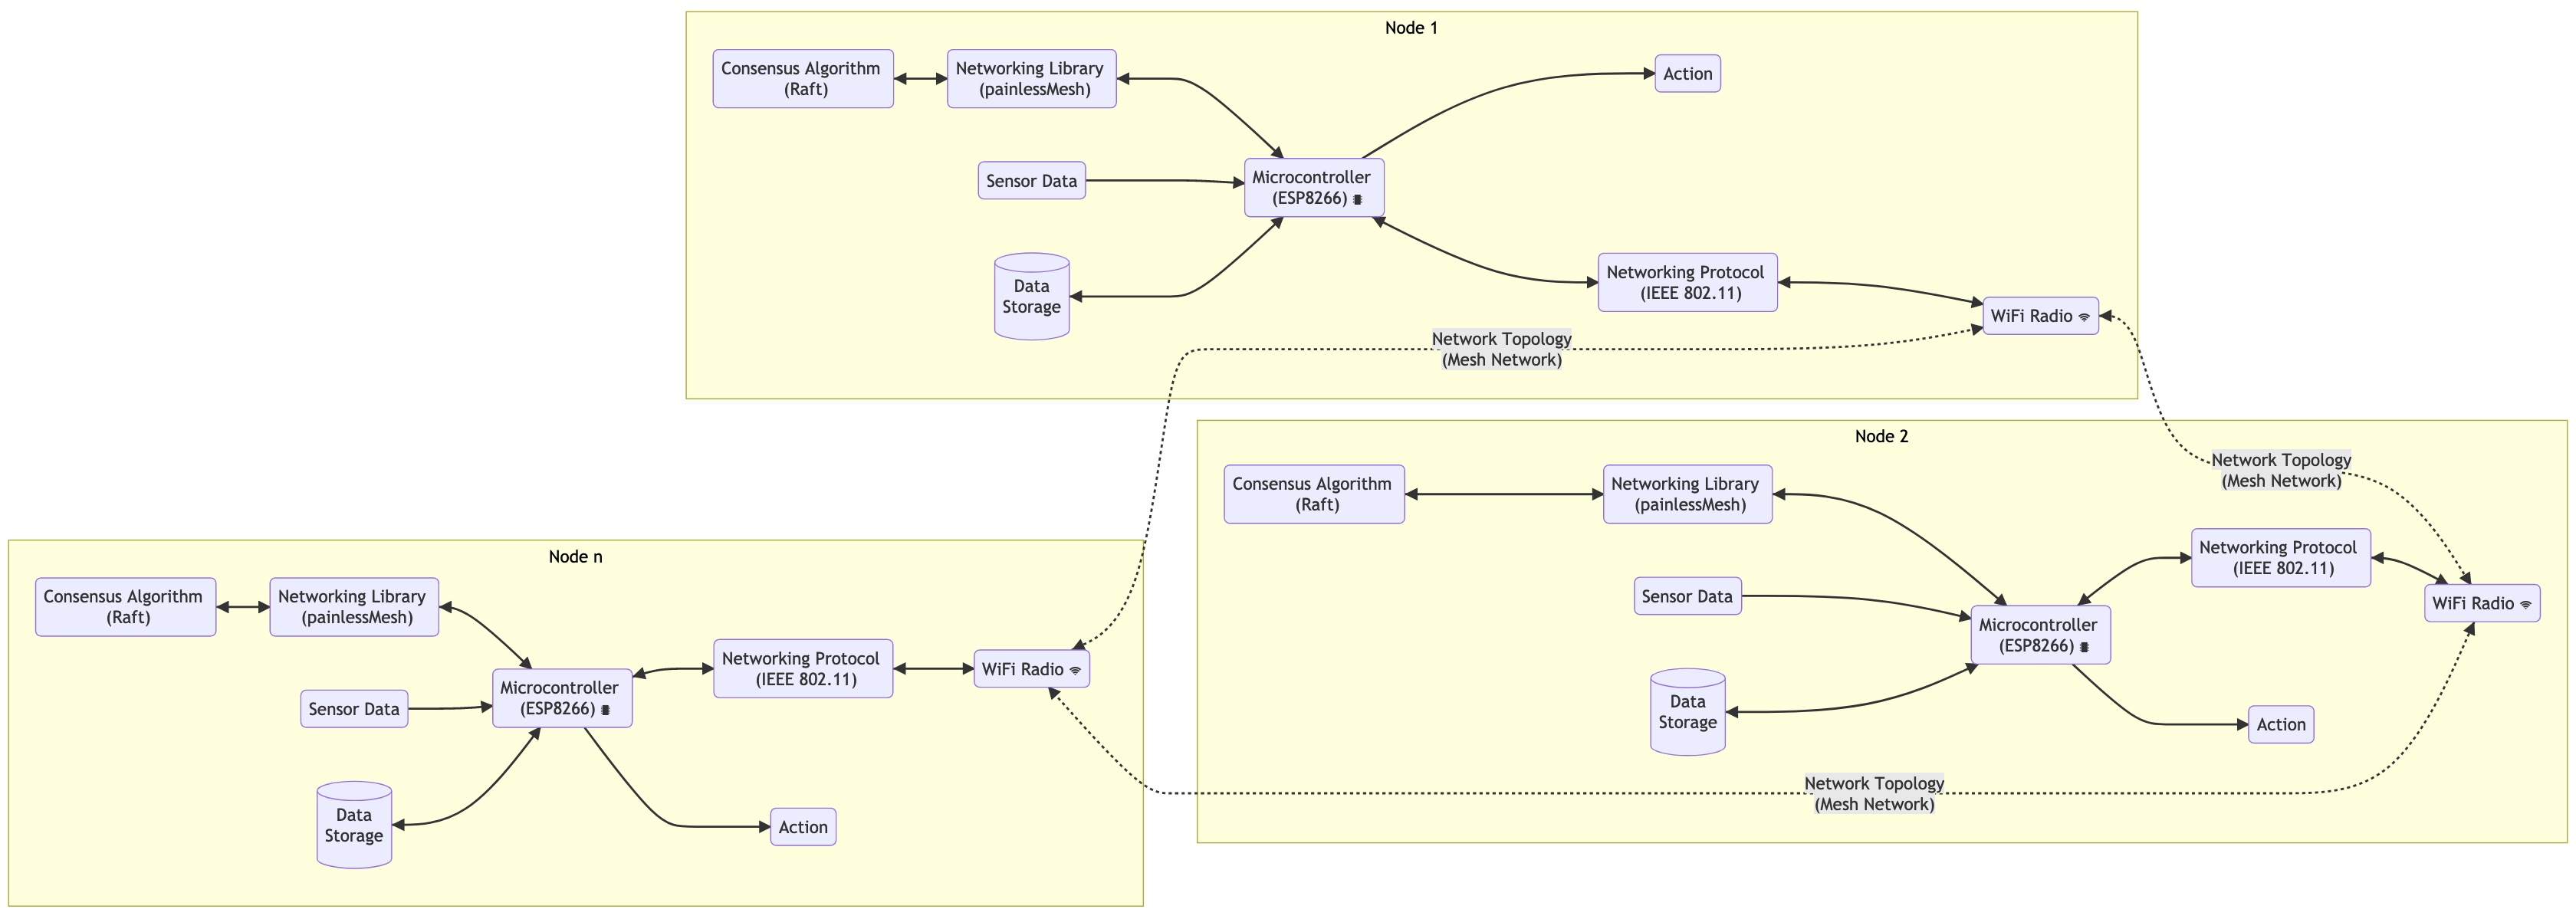
\includegraphics[width=1\textwidth]{final-proposal/images/final_design_nodes.png}
    \caption{Detailed black box of each node in the final design}
    \label{fig:final_design_node_bb}
    
% flowchart LR
%     1_radio  <-..-> |"Network Topology <br> (Mesh Network)"| 2_radio
%     2_radio <-.....->  |"Network Topology <br> (Mesh Network)"| n_radio
%     n_radio <-..->  |"Network Topology <br> (Mesh Network)"| 1_radio

%     subgraph 1[Node 1]
%       1_radio(WiFi Radio fa:fa-wifi)
%       1_cons("Consensus Algorithm <br> (Raft)")
%       1_netProc("Networking Protocol <br> (IEEE 802.11)")
%       1_netLib("Networking Library <br> (painlessMesh)")
%       1_cont("Microcontroller <br> (ESP8266) fa:fa-microchip")
%       1_act(Action)
%       1_sens(Sensor Data)
%       1_sto[(Data <br> Storage)]
%       1_sto <--> 1_cont
%       1_sens --> 1_cont
%       1_cont --> 1_act
%       1_cons <--> 1_netLib <--> 1_cont <--> 1_netProc <--> 1_radio
%     end

%     subgraph 2[Node 2]
%       2_radio(WiFi Radio fa:fa-wifi)
%       2_cons("Consensus Algorithm <br> (Raft)")
%       2_netProc("Networking Protocol <br> (IEEE 802.11)")
%       2_netLib("Networking Library <br> (painlessMesh)")
%       2_cont("Microcontroller <br> (ESP8266) fa:fa-microchip")
%       2_act(Action)
%       2_sens(Sensor Data)
%       2_sto[(Data <br> Storage)]
     
%       2_cons <--> 2_netLib <--> 2_cont <--> 2_netProc <--> 2_radio
%       2_sto <--> 2_cont
%       2_sens --> 2_cont
%       2_cont --> 2_act
%     end

%     subgraph n[Node n]
%       n_radio(WiFi Radio fa:fa-wifi)
%       n_cons("Consensus Algorithm <br> (Raft)")
%       n_netProc("Networking Protocol <br> (IEEE 802.11)")
%       n_netLib("Networking Library <br> (painlessMesh)")
%       n_cont("Microcontroller <br> (ESP8266) fa:fa-microchip")
%       n_act(Action)
%       n_sens(Sensor Data)
%       n_sto[(Data <br> Storage)]
%       n_sto <--> n_cont
%       n_sens --> n_cont
%       n_cons <--> n_netLib <--> n_cont <--> n_netProc <--> n_radio
%       n_cont --> n_act
      
%     end
\end{figure}


%%%%%%%%%%%%%%%%%%%%%%%%%%%%%%%%%%%%%%%%%%%%%%%%%%%%%%%
\vspace{-25pt}
\subsection{Microcontroller}
The final design will use ESP8266 microcontrollers to run the required consensus algorithm and perform the networking functionality with its built-in IEEE 802.11 based WiFi module. As a part of the hardware demonstration, additional peripherals will be connected to the ESP8266 microcontroller. This will demonstrate the capabilities of the consensus algorithm on a mesh network by transferring information across the network. Figure \ref{fig:final_design_prototype} shows the block diagram for the peripherals that will be connected to the microcontroller on each node. The peripherals will help measure the performance of our software library and evaluate against the design criteria \& constraints defined in the previous sections of this report.

\begin{figure}[H]
    \centering
    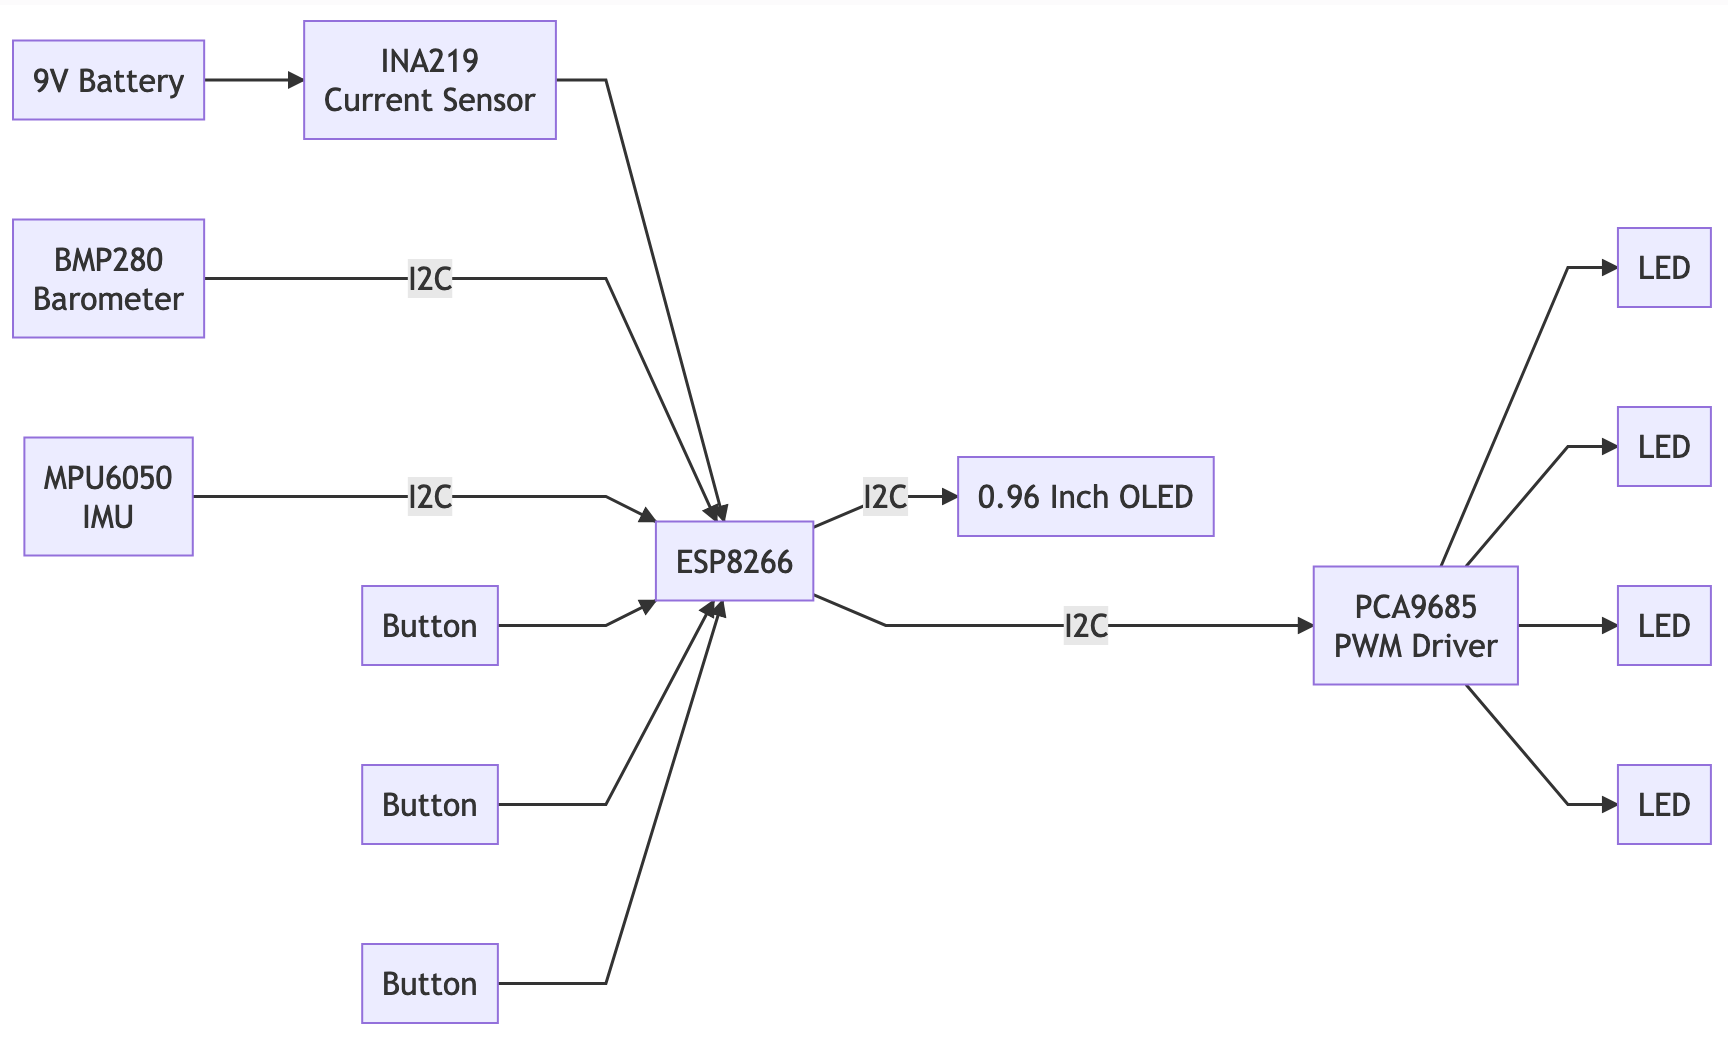
\includegraphics[width=0.5\textwidth]{final-proposal/images/final_design_prototype.png}
    \caption{Block diagram for the hardware demonstration of the project}
    \label{fig:final_design_prototype}
    
% graph LR
%   battery[9V Battery] --> curr
%   curr[INA219 <br> Current Sensor] --> esp[ESP8266]
%   baro[BMP280 <br> Barometer] ---> |I2C| esp
%   imu[MPU6050 <br> IMU] ---> |I2C| esp

%   esp ---> |I2C| pwm[PCA9685 <br> PWM Driver]
%   pwm --> led1[LED]
%   pwm --> led2[LED]
%   pwm --> led3[LED]
%   pwm --> led4[LED]

%   button1[Button] --> esp
%   button2[Button] --> esp
%   button3[Button] --> esp
  
%   esp --> |I2C| oled[0.96 Inch OLED]
\end{figure}


%%%%%%%%%%%%%%%%%%%%%%%%%%%%%%%%%%%%%%%%%%%%%%%%%%%%%%%
\subsection{Consensus Algorithm and Networking}
The final design is expected to rely upon painlessMesh and the Raft consensus algorithm. We will use painlessMesh as the mesh networking library to relay the election and log replication messages among the nodes. For clarity, we split both these flows into two figures.

Figure \ref{fig:flow} shows the logical flow of the firmware running on each node. All of the nodes in the network will initialize a mesh network using painlessMesh and then switch to the follower state. Following the Raft algorithm, a leader node will be selected through an election process. Any new nodes will autonomously be added to the network by the painlessMesh library and will default to follower mode until they declare candidacy.

\begin{figure}[H]
    \centering
    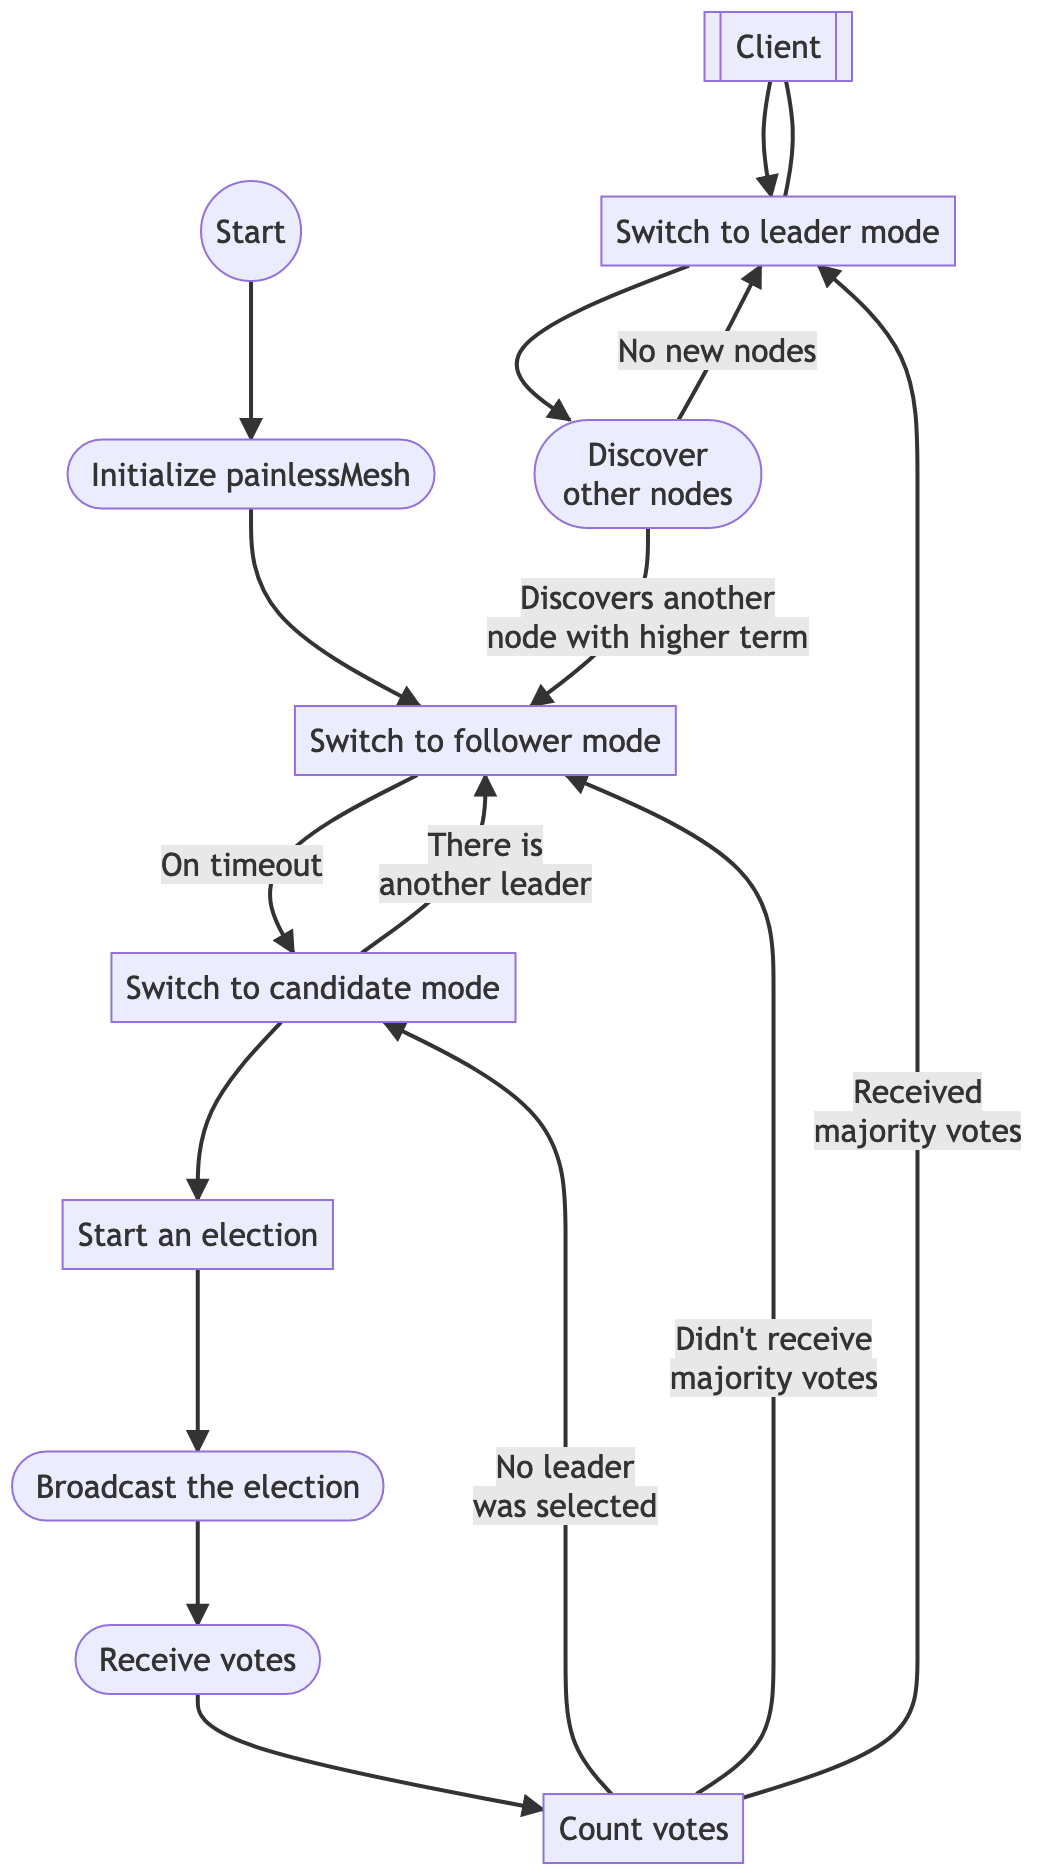
\includegraphics[width=0.53\textwidth]{final-proposal/images/final_design.png}
    \caption{Software logic}
    \label{fig:flow}

% flowchart TD
%   client[[Client]]
%   start((Start))

%   init([Initialize painlessMesh])
%   broadcast([Broadcast the election])
%   receive([Receive votes])
%   discover([Discover <br> other nodes])

%   follower[Switch to follower mode]
%   elect[Start an election]
%   candidate[Switch to candidate mode]
%   leader[Switch to leader mode]
%   count[Count votes]

%   start --> init
%   init --> follower
%   follower --> |On timeout| candidate
%   candidate --> elect
%   candidate --> |There is <br>another leader| follower
%   elect --> broadcast
%   broadcast --> receive
%   receive --> count
%   count --> |No leader <br> was selected| candidate
%   count --> |Didn't receive <br> majority votes| follower
%   count --> |Received <br>majority votes| leader

%   leader --> discover
%   discover --> |No new nodes| leader
%   discover --> |Discovers another <br> node with higher term| follower

%   client --> leader
%   leader --> client
\end{figure}

Figure \ref{fig:data_flow} shows three nodes replicating the logs to achieve consensus. Since Raft's primary goal is to achieve data consensus, we see that the leader node waits for confirmation whenever it communicates a change in data to a follower node. Once again, we will use the broadcast capabilities of the painlessMesh networking library to communicate between nodes as well as store the data received from communication onto the device's local storage. This data replication occurs in conjunction with the leader election process.

\begin{figure}[H]
    \centering
    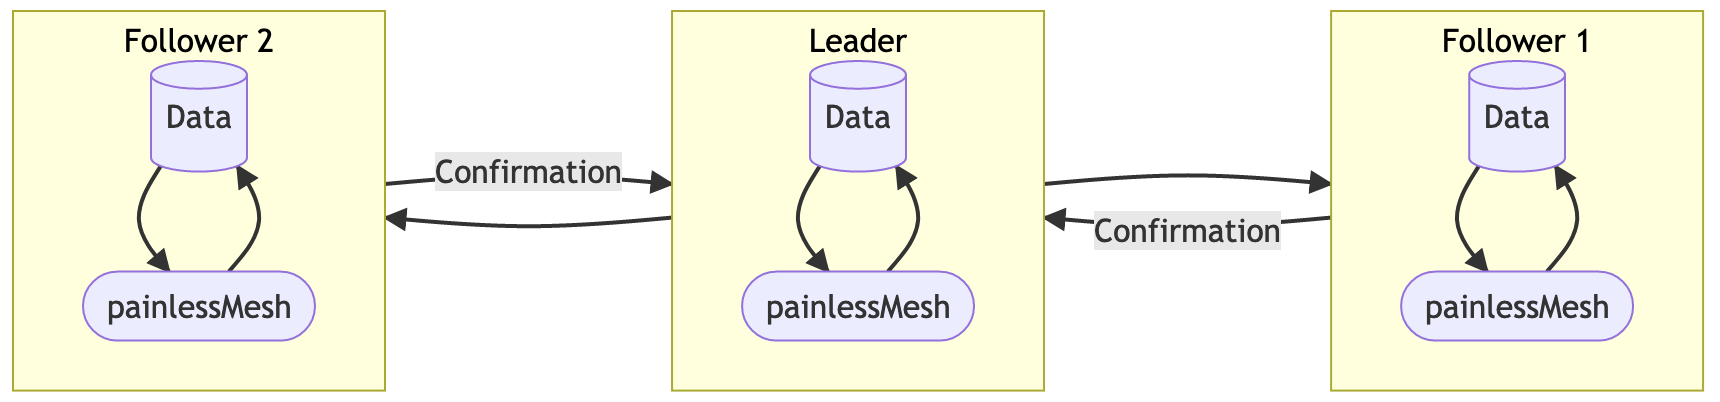
\includegraphics[width=0.7\textwidth]{final-proposal/images/final_design_data.png}
    \caption{Data flow between leader and follower nodes}
    \label{fig:data_flow}
    
% flowchart LR
%   subgraph Leader
%     data[(Data)]
%     painlessMesh([painlessMesh])
%     data --> painlessMesh --> data
%   end

%   subgraph Follower_1[Follower 1]
%     f_1_data[(Data)]
%     f_1_painlessMesh([painlessMesh])
%     f_1_data --> f_1_painlessMesh --> f_1_data
%   end

%   subgraph Follower_2[Follower 2]
%     f_2_data[(Data)]
%     f_2_painlessMesh([painlessMesh])
%     f_2_data --> f_2_painlessMesh --> f_2_data
%   end
  
%   Leader --> Follower_2
%   Leader --> Follower_1
%   Follower_1 --> |Confirmation| Leader
%   Follower_2 --> |Confirmation| Leader
\end{figure}




 
 